\chapter{Environment}
\label{chapter:environment}

\section{Multi-access Edge Computing}

\subsection{Far Edge Cloud}



Benefits of far edge
    - Latency
    - Allowing thin clients / offloading task to edge
    - Price and effect to environment
    - Security
    - Centralized repairing / upgrading
    - Less power consumption
    

\begin{figure}[ht]
  \begin{center}
    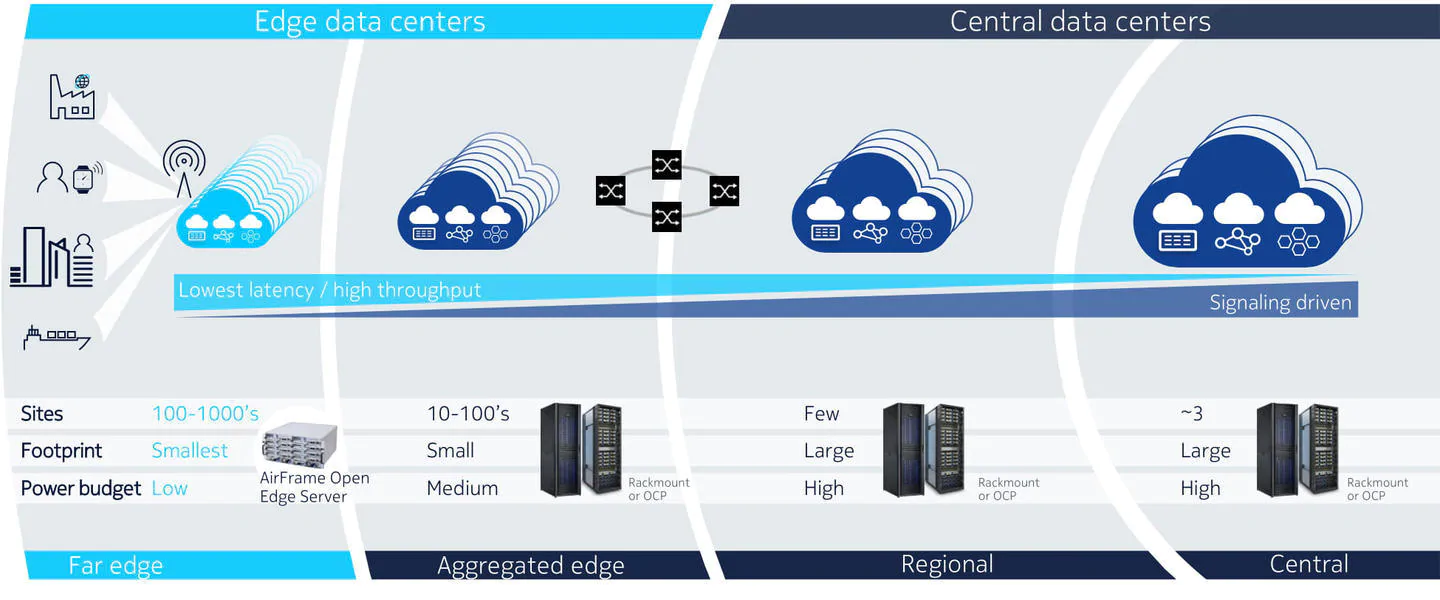
\includegraphics[width=13.5cm]{LaTeX/images/AirFrameOpenEdgeServer.png}
    \caption{Far edge comparison to central data center \cite{AirFrameOpenEdgeServer}}
    \label{fig:AirFrameOpenEdgeServer}
  \end{center}
\end{figure}

\subsection{Applications}


\subsection{SR-IOV}
\label{section:SR-IOV}

I/O performance is critical to high performance telco systems. I/O intensive servers may waste CPU cycles, waiting for I/O data or spinning on idle cycles, which reduces system performance and increases latency. Single Root I/O Virtualization (SR-IOV) standard allows an I/O device, such as network interface controller (NIC), to be shared by multiple VMs. The SR-IOV technology is a hardware based virtualization solution that improves both performance and scalability. \cite{Dong2012}

Traditionally, when a guest accesses the I/O device, VMM needs to intervene in the data processing to share the physical device. The VMM intervention leads to additional I/O overhead for a guest OS. SR-IOV provides hardware enhancements for the Peripheral Component Interconnect Express (PCIe) device, which aims to remove major VMM intervention for performance data movement, such as the packet classification and address translation. An SR-IOV-capable device is able to create multiple light-weight instances of PCI function entities, known as Virtual Functions (VF). Each VF can be assigned to a VM for direct access, but still shares major device resources, achieving both resource sharing and high performance. \cite{Dong2012}





Requirements
- Root
- SR-IOV
- NICS

- Environment in MEC application
    - How migrated?
    - Elevated privileges and other requirements compared
    - Something else?
Nokia's environment \\
Usage of KC in Nokia's environment \\





% Comment: If your sentence ends in a capital letter write \@ before the period

% If you do need a normal space after a period (instead of
% the longer sentence separator), use \  (backslash and space) after the
% period. Like so: a.\ first item, b.\ second item.